\documentclass[a4paper,kul]{kulakarticle} %options: kul or kulak (default)

\usepackage[utf8]{inputenc}
\usepackage[dutch]{babel}
\usepackage{float}
\usepackage{subcaption}

\date{Academiejaar 2019 -- 2020}
\address{
  Faculteit Industriële Ingenieurswetenschappen \\
  Systeemontwerp met HDL \\
  S. Verslype}
\title{Verslag spectrogram}
\author{Robin Nollet, Sebastian Vantomme, Ine Vanderhaeghe}


\begin{document}
	
\maketitle
	
\begin{center}
	\centering
	\vspace*{\fill}
	\huge
	\textbf{Verslag: bouwen van een spectrogram op een FPGA met behulp van de VHDL-taal}
	\vspace*{\fill}
\end{center}
	
\newpage
	
\tableofcontents

\newpage

\section{Probleemstelling: een audiospectrogram}

Doorheen het semester hebben we ons met ons groepje bezig gehouden met het bouwen van een audiospectrogram.

\subsection{Wat is een spectrogram?}

Het kan handig zijn om snel de frequentieinhoud van een signaal te zien, naar analyse toe. Gezien een signaal ook vaak veranderlijk is in de tijd, kan ook de frequentieinhoud veranderen in functie van de tijd. Er bestaat een methode om de frequentieinhoud van een signaal weer te geven in functie van de tijd. Dit heet een \textit{Spectrogram}. Een spectrogram kan goed samengevat worden volgens de volgende definitie: het is een visuele representatie van de energie in elke frequentie uitgezet in de tijd. Een spectrogram heeft verschillende toepassingen. Enkele voorbeelden hiervan is bv. in de audio, of in de analyse van licht. Dit project focust specifiek op het analyseren van audiosignalen, hoorbaar voor het menselijk oor. Hiervoor nemen we standaard een range van $20Hz$ tot $20kHz$. In de audiowereld worden deze frequenties vaak de \textit{pitch} genoemd van het signaal. 


Mogelijke toepassingen van een spectrogram die hoorbare audiosignalen worden hieronder opgesomt:
\begin{itemize}
	\item analyse van Muziek(-instrumenten)
	\item analyse van Spraak
	\item analyse van Dierengeluiden
	\item analyse van RF modulatietechnieken
\end{itemize}

\subsection{Hoe wordt een spectrogram voorgesteld?}

De grafische voorstelling van een spectrogram zou eigenlijk in 3 dimensies moeten gegeven worden. Dit is echter wat lastig om dan op één oogopslag informatie te kunnen uit aflezen. Daarom worden in de literatuur vaak de volgende afspraken gevolgd:
\begin{itemize}
	\item De tijd wordt op de horizontale as uitgezet;
	\item De frequentie wordt op de verticale as uitgezet;
	\item De sterkte van de frequentie wordt vaak weergegeven met behulp van kleurintensiteit of een kleurgradiënt.
\end{itemize}
In figuur \ref{fig:typischegrafischevoorstellingspectrogram} is een typische grafische voorstelling gegeven.

\begin{figure}[H]
	\centering
	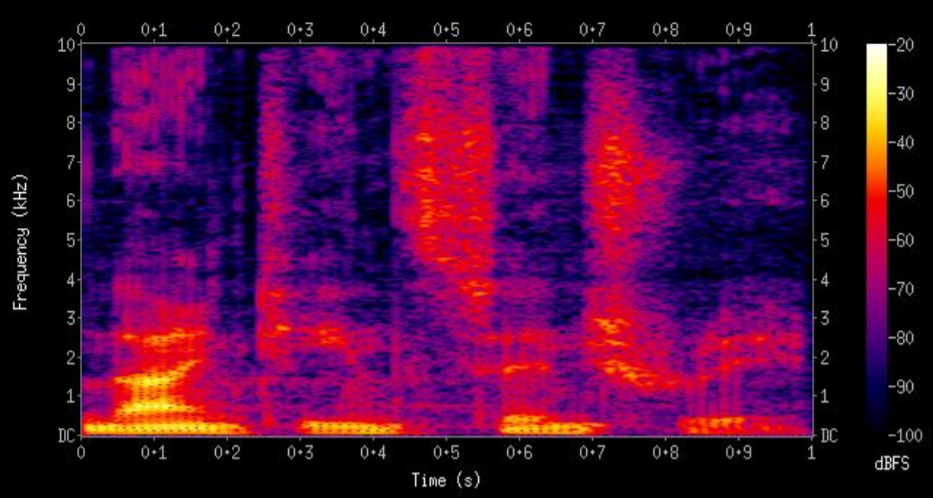
\includegraphics[width=0.7\linewidth]{typischeGrafischeVoorstellingSpectrogram.png}
	\caption{Een typische grafische voorstelling van een spectrogram}
	\label{fig:typischegrafischevoorstellingspectrogram}
\end{figure}

\subsection{Gebruikte methoden om een spectrogram te implementeren}

In de literatuur kunnen 2 veelgebruikte methoden voor de implementatie van een Spectrogram gevonden worden.
\begin{enumerate}
	\item Met behulp van de FFT: van het ingenomen signaal wordt de \textit{Fast Fourier Transform (FFT)} genomen, wat een versnelde versie is van de \textit{Discrete Fourier Transform (DFT)}. Dit toont de frequentieinhoud van het signaal. Een belangrijke eigenschap van deze transformatie is dat ze een discrete ingang (de audio) en een discrete uitgang (de frequentieinhoud van dit signaal) heeft. 
	\item Met behulp van een filterbank: hier wordt een reeks banddoorlaatfilters geïmplementeerd, die allemaal op hetzelfde signaal werken. Door na iedere filter dan te gaan kijken wat de energie van het signaal is, kan dit als een maat gebruikt worden voor de frequentieinhoud van ons ingangssignaal.
\end{enumerate}

Naar implementatie toe heeft men dan een keuze, dit hangt af welke resolutie men wilt in de frequentie. Wil men een grote resolutie in de frequentie, gaat men eerder kiezen voor de aanpak met de FFT. Als men met een lage frequentieresolutie zich tevreden kan nemen, wordt er vaak geopteerd voor de implementatie met die meerdere filters.\\
Wij hebben hier gekozen voor de implementatie met een FFT, omdat deze een stuk flexibeler is in implementatie.


\subsection{Afwerkingsgraad}

Onze opdracht bestaat er uit om zelf een real-time spectrogram te maken van een audiosignaal dat aangeboden wordt door een FPGA. Dit spectrogram moet gevisualiseerd worden op een extern scherm via VGA of HDMI. \\

Als eerste moet er dus een analoog audiosignaal kunnen binnengelezen worden via de audiocodec chip. Deze zorgt zelf voor de digitalisatie van het signaal en geeft dit door aan de FPGA. Er moet dus communicatie mogelijk zijn tussen de codec chip en de FPGA. \\
Daarna moet het spectrum bepaald kunnen worden. Er worden een aantal samples genomen op het gedigitaliseerde audiosignaal. Daarop wordt een FFT uitgevoerd. Hierbij kan gewerkt worden met aansluitende of overlappende blokken van de samples. Als met overlapping gewerkt wordt zou de resolutie fijner zijn, maar het zou ook complexer zijn. \\
Ten laatste moet de verzamelde data na de FFT op een 2D map komen die het spectrogram voorsteld. Eens het volledige scherm gevuld is, moet de oudste meting verwijderd worden en schuift het spectrogram een tijdseenheid op via een FIFO. \\

In het volledige systeem moet rekening gehouden worden met de timing en mogelijke asynchrone signalen. \\

Er zal tijdens de evaluatie van het project met verschillende testsignalen gecontroleerd worden als het project juist ontworpen is. Voorbeelden van testsignalen zijn FM modulatie, frequentie sweep, blokgolf, DTMF signalen, ... \\
\\ Er zijn enkele minimum vereisten in dit project:
\begin{itemize}
	\item Er wordt gewerkt met een FPGA bord naar keuze (Zedboard, Zybo, PYNQ, ...)
	\item Interface met audiocodec chip
	\item Real-time FFT op audio input
	\begin{itemize}
		\item 1 kanaal (mono)
		\item Aansluitende blokken van \textit{N} samples
	\end{itemize}
	\item Opstellen en updaten van spectrogram
	\item VGA/HDMI interface logica
	\item Beschikbaar stellen van spectrogram op een extern beeldscherm
\end{itemize}
Daarnaast zijn nog enkele mogelijkheden tot uitbreiding:
\begin{itemize}
	\item Stereo spectrogram
	\item FFT op overlappende tijdssignalen
	\item 3D spectrogram
	\begin{itemize}
		\item Amplitude als kleurintensiteit
	\end{itemize}
	\item Full HD
	\item Audio loopback
	\begin{itemize}
		\item Signaal terug naar buiten via line-out of headphone
	\end{itemize}
\end{itemize}

\section{Oplossingsstructuur}
Voor dergelijke probleemstelling is de eerste stap om een \textit{pipeline} op te stellen, een stappenplan van wat er met de data moet gebeuren van input tot aan output. Bij deze opdracht hebben we de pipeline toegepast gevonden in figuur \ref{fig:toegepastePipeline}.

\begin{figure}[H]
	\centering
	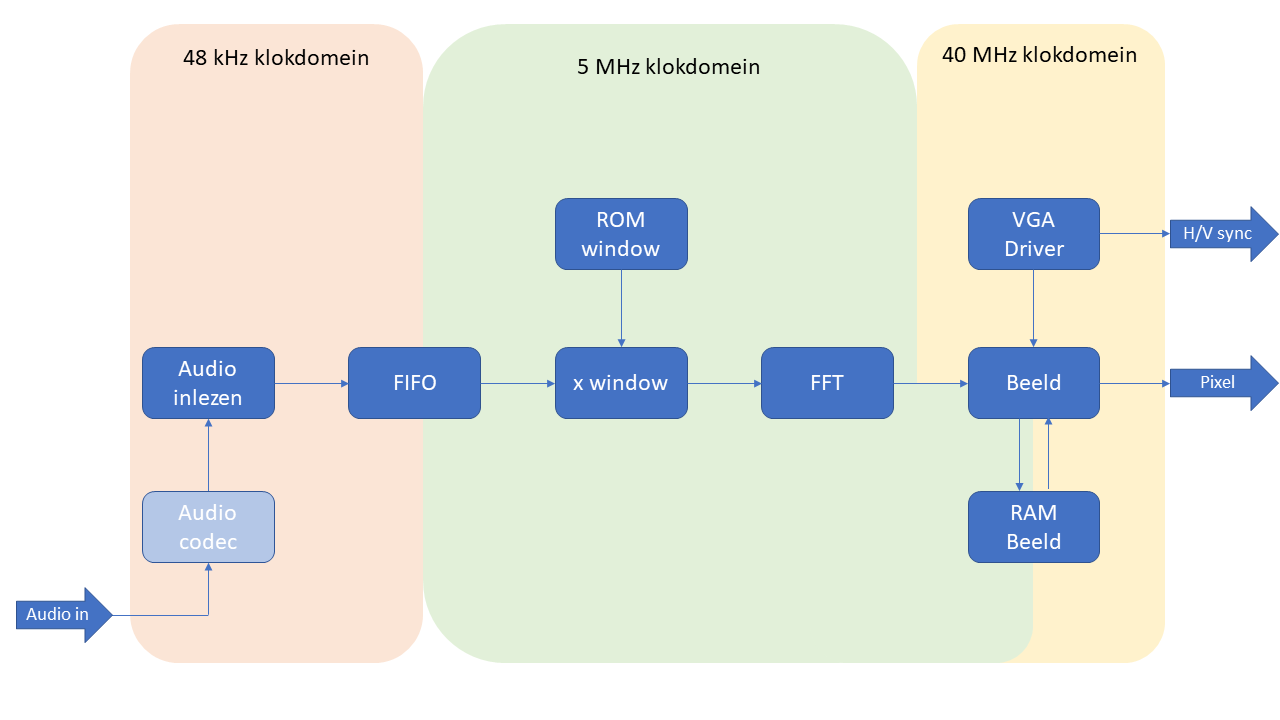
\includegraphics[width=0.7\linewidth]{Pipeline.png}
	\caption{toegepaste pipeline}
	\label{fig:toegepastePipeline}
\end{figure}

Zoals te zien valt op de figuur is het werk grotendeels op te splitsen in 3 grote delen, namelijk aan de hand van het klokdomein. Er hoeft dan gewoon via een dual-port-RAM een overschakeling te worden gemaakt tussen deze verschillende klokdomeinen. We hebben het werk opgesplitst in de volgende delen:

\begin{enumerate}
	\item Audio inlezen. Kort samengevat is dit het inlezen van de audio via de audiocodec en stockeren in de FIFO.
	\item Fourier nemen. Dit is de data uit de FIFO halen, er een window op toepassen en er daarna de fouriertransformatie op loslaten. De output van de FFT wordt dan doorgegeven aan Beeld.
	\item Grafisch weergeven. Hier wordt de data gegeven van de FFT opgeslagen in een RAM, die dan ook wordt uitgelezen aan een andere kloksnelheid. Zo wordt de data visueel op het scherm gerepresenteerd.
\end{enumerate}

\subsection{Audiocodec}

Om de audio binnen te lezen, zijn er 2 belangrijke bestanden: \textit{adau1761} en \textit{audio\_if}. Deze bestanden lezen de data binnen en genereren daar de juiste clock signalen voor. In het top level wordt daar dan een audio loopback van gemaakt om de data die binnengelezen werd ook weer naar buiten te sturen. De data die binnengelezen werd wordt ook naar een FIFO gestuurd, zodat deze op de juiste momenten binnengelezen kan worden in de FFT controller.

\subsection{Fourieranalyse}

De FFT-controller bevat drie componenten, namelijk: een FFT ip, een window en een multiplier. In de FFT ip wordt de FFT van het signaal genomen. De window is een blok geheugen met daarin een Hanning window. De data die afkomstig is van een FIFO-geheugen wordt vermenigvuldigd met dit window. Deze vermenigvuldiging gebeurt in de multiplier ip.

\subsection{Grafisch weergeven}
Om de berekende resultaten dan ook grafisch weer te geven, hebben we gebruik gemaakt van VGA. Om dit wat beter beheersbaar te houden is de architectuur opgesplitst in \textit{VGA\_Driver} en \textit{mem\_interface\_Beeld}.\\
\textit{VGA\_Driver} heeft als functie om Hsync en Vsync te genereren. Daarnaast genereert het ook een X en Y, wat de huidige positie is van de pixel die moet worden doorgestuurd, tesamen met een flag die hoog komt als men in het actieve gebied zit van het beeld (dus niet in de porch of syncpulses).\\
\textit{mem\_interface\_Beeld} zorgt met de gegeven X en Y waarde dat de juiste pixel naar buiten komt. Ook zorgt het voor de overschakeling tussen de verschillende klokdomeinen.

\section{Implementatie}
%Algemeen overzicht

\begin{figure}[H]
	\centering
	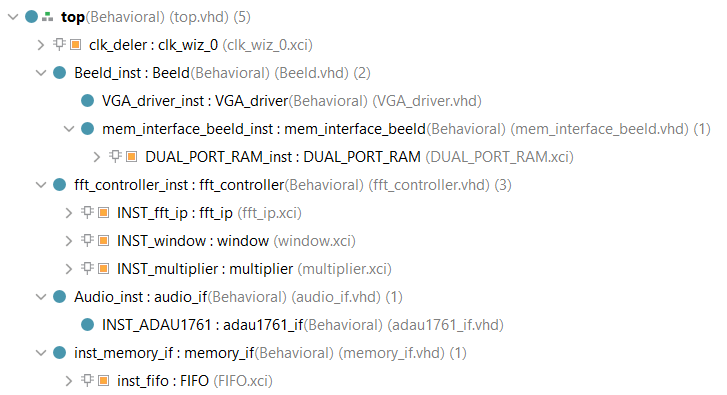
\includegraphics[width=0.7\linewidth]{HierarchieVivado.png}
	\caption{Hierarchie van de implementatie}
	\label{fig:hierarchieVivado}
\end{figure}

Zoals te zien is op deze figuur is er een top laag die alle andere onderdelen met elkaar verbindt. Hier wordt een klok deler gemaakt, zodat elk onderdeel in zijn eigen klokdomein kan werken. \\

Voor het beeld is een VGA driver nodig en een memory interface. Dit is een dual port ram, omdat de data die er in geschreven wordt niet op dezelfde klok werkt als de data die er uit gelezen wordt. Het schrijven gebeurt door de FFT controller, het lezen door de beeld interface. \\

De FFT controller maakt gebruikt van 3 IP's: een om de FFT te berekenen, een die het window bevat die moet vermenigvuldigd worden met de waarden die uit de FFT komen en een die de andere 2 vermenigvuldigd met elkaar. \\

De audio interface maakt gebruik van een driver voor de \textit{adau1761} chip die op de FPGA aanwezig is.\\

Daarnaast is ook een memory interface. Deze maakt gebruikt van een FIFO die op 2 verschillende klokken werkt. Hier wordt de data doorgegeven tussen de audio interface en de FFT controller. De audio interface zal data in de FIFO schrijven volgens een klok die ze zelf genereerd, de FFT controller leest ze uit wanneer het geheugen vol is op een klok die sneller is dan die van de audio interface.

\subsection{Audiocodec}

Er kan gebruik gemaakt worden van de audiocodec die aanwezig is op het Zedboard. Dit is de \textit{adau1761}. Hiervoor moest een driver geschreven worden. Voor ons project hebben we een driver kunnen gebruiken die we gekregen hadden van Dhr. Verslype. Deze driver krijgt zowel serieel als parallelle data binnen. De samples van het linker en rechter kanaal zijn 24 bit breed. Deze worden verwerkt in de driver en er wordt een linker en rechter output gegenereerd die 24 bit breed zijn en een seriële data output. \newline

Daarnaast moest een interface geschreven worden die de clock genereerd en de data die de driver binnenleest op een juiste manier door geeft naar het top level. Ook hier hebben we gebruik gemaakt van een interface die we gekregen hadden van Dhr. Verslype. Deze interface heeft een kloksignaal nodig van 100 MHz en 12,288 MHz. Deze genereren 3 nieuwe kloksignalen: de \textit{master clock}, de \textit{digital audio bit clock} en de \textit{digital audio left-right clock}. Deze worden gebruikt in de adau1761 codec. \newline

De configuratie van de audio interface werkt met het $I^2C$ protocol, het doorgeven van audio data gebeurt via het $I^2S$ protocol.\newline

In het top level wordt daarna een audio loopback gemaakt. De data wordt ook doorgegeven aan een FIFO memory, zodat deze uitgelezen kan worden door de FFT controller. Het geheugen is 2048 waarden groot, dus wanneer deze vol is wordt een flag hoog gezet zodat de FFT controller weet dat alle waarden die in de memory staan geldig zijn. Het adres waarop de data geschreven moet worden in de FIFO wordt gegenereerd door middel van een counter tussen 0 en 2048. 

\subsection{Fourieranalyse}

De FFT wordt berekend met behulp van de “Fast Fourier Transform v9.1 LogiCORE IP”. De gesampelde waarden komen uit een geheugen met een FIFO-structuur. Deze samples worden nog vermenigvuldigd met een window alvorens ze gebruikt worden in de FFT. De window is opgeslagen in een gelijkaardig geheugen als de FIFO. Deze twee hebben dezelfde latency.

\begin{figure}[H]
	\centering
	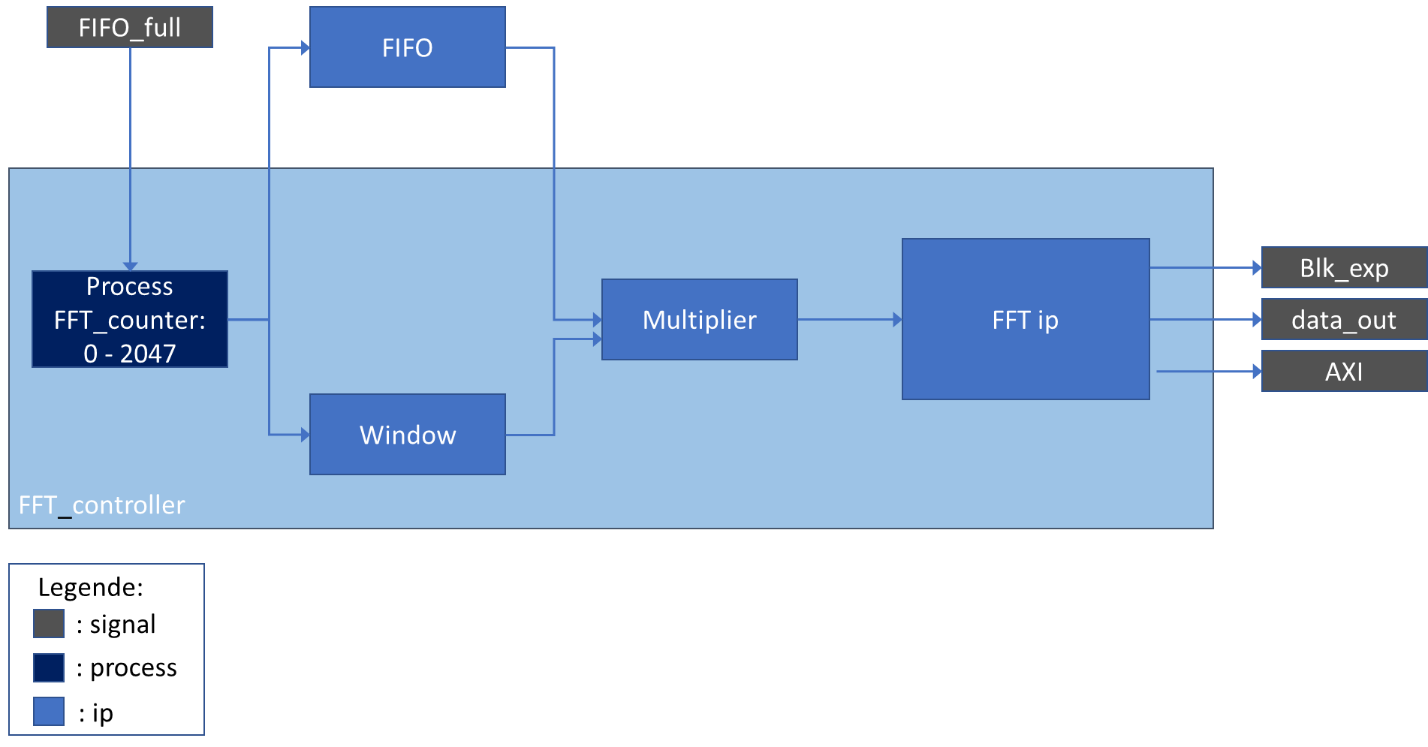
\includegraphics[width=0.7\linewidth]{FFT_controller.png}
	\caption{FFT controller}
	\label{fig:fft_controller}
\end{figure}

De FFT ip maakt gebruik van de “Radix-4 Burst I/O” architectuur. Hierbij moet een frame volledig naar buiten gebracht zijn voordat een nieuw frame verwerkt kan worden. Dit zorgt voor de noodzaak om te werken op een hogere frequentie dan de sample frequentie van de ingang. Dit zorgt voor de noodzaak van een buffer tussen de audio interface en de FFT ip. Dit wordt opgelost met het FIFO-geheugen.

Tijdens het berekenen van de FFT van het signaal moet de data soms geschaald worden. Dit gebeurt met een block exponent. Hierbij wordt de data zodanig geschaald dat de uitgang een full scale heeft. Deze oplossing zorgt ervoor dat de besturing van de FFT gemakkelijker wordt.\\

De uitgang bestaat uit 7 bits, terwijl de ingang 24 bits breed is. De ingang heeft deze breedte omdat de audio codec deze breedte gebruikt. Normaal is de breedte van een FFT even breed als de ingang. Maar gezien de frames uit de FFT moeten opgeslagen worden in een blok geheugen was er de noodzaak om de resolutie te verlagen naar 7 bits. De uitgang wordt gehaald uit het reëel deel van de uitgang. De uitgang van het reëel deel van de FFT ip is 24 bits breed, daarvan worden de bovenste 4 bits en de onderste 13 bits genegeerd. De bovenste 4 bits worden niet bekeken omdat gebleken is dat deze toch telkens nul zijn.

De block exponent zorgt ervoor dat de uitgang altijd full scale is. Wanneer er enkel ruis in het data signaal aanwezig is, zou dit ook full scale uit de uitgang komen.  In de uitgang resideert de ruis echter nog steeds enkel in de minst significante bits. Gezien de minst significante bits niet bekeken worden is het scherm zo goed als perfect zwart wanneer er enkel ruis aanwezig is aan de ingang.
Het reëel deel van een spectrum zal altijd symmetrisch zijn. Het volstaat dus enkel de helft van het spectrum weer te geven. Dit is ook wat hier gedaan wordt. Enkel de eerste helft van het reëel deel wordt doorgegeven aan het beeldverwerking gedeelte, zo wordt enkel dit deel geplot.\\

Wanneer het geheugen bijna vol is maakt de audio interface een signaal FIFO-full hoog. Dit geeft aan dat het geheugen bijna vol is. Dit signaal wordt gesampled in de FFT-controller. Nadat gemerkt wordt dat dit signaal hoog is begint het proces FFT-counter. Hierin wordt er geteld van 0 tot 2047, dit is de grootte van een frame. Deze teller wordt gebruikt als geheugen adres voor de FIFO en het window. De data die uit deze twee blokken komt wordt vermenigvuldigd met elkaar. Zo wordt een ge-windowed signaal bekomen.\\

Om spectral leakage te voorkomen wordt een window gebruikt. Het gekozen window is een Hanning window. Een Hanning window is een window die best gebruikt wordt wanneer er vooraf geen kennis is over het signaal. Dit is hier het geval gezien we alles uit het audio spectrum willen kunnen afbeelden.
(Bron: National Instruments, „Understanding FFTs and Windowing,” [Online]. Available: http://download.ni.com/evaluation/pxi/Understanding%20FFTs%20and%20Windowing.pdf. [Geopend 17 Dec. 2019].)


\subsection{Grafisch weergeven}
Om de berekende resultaten dan ook grafisch weer te geven, hebben we gebruik gemaakt van VGA. Om dit wat beter beheersbaar te houden is de architectuur opgesplitst in \textit{VGA\_Driver} en \textit{mem\_interface\_Beeld}.\\

\textit{VGA\_Driver} genereert Hsync en Vsync. Dit werkt vrij eenvoudig door 2 tellertjes bij te houden (in de code \textit{Hteller} en \textit{Vteller}). Deze tellertjes geven weer waar op welke horizontale lijn men zit, alsook de positie in de lijn. Zo wordt het scherm horizontaal van links naar rechts doorlopen, en per lijn van boven naar beneden. Het is vrij eenvoudig om zo de Hsync en Vsync pulses te genereren, door enkel gewoon te gaan kijken wat de waarde is van de respectievelijke tellers.\\
Extra uitgangen van dit blokje zijn VGA\_X en VGA\_Y, die de huidige positie is van de pixel die moet worden doorgestuurd. Erg eenvoudig, want hiervoor moeten we gewoon de tellertjes die Hsync en Vsync genereren naar buiten sturen. Ook wordt een flag gegenereert, die hoog komt als men in het actieve gebied zit van het beeld (dus niet in de porch of syncpulses).\\


\textit{mem\_interface\_Beeld} zorgt voor de overschakeling tussen klokdomeinen en het beheer van de data bij uitlezen en schrijven. Hierin is de functionaliteit opgesplitst in 3 delen:
\begin{itemize}
	\item Memory component: voor de overschakeling tussen de klokdomeinen hebben we gebruik gemaakt van een dual port RAM, een stuk geheugen die langs 1 kant met een bepaalde klok geschreven wordt, en langs de andere kant wordt uitgelezen met een andere klok. Qua adressering loopt dit geheugen in dezelfde richting als de VGA: eerst van links naar rechts horizontaal, daarna lijntje per lijntje verticaal. Daardoor heeft de linkerbovenhoek dus het laagste adres, en de rechterbovenhoek het hoogste adres. Om dit adres wat te gaan abstraheren, hebben we dit opgesplitst in een $X$ en een $Y$. Het adres valt dan te berekenen via de volgende formule:
	
	$$ A = X + lijnbreedte \times Y $$
	
	met $X$ de horizontale pixelpositie, $Y$ de verticale pixelpositie en $A$ het adres.
	
	\item Writing to memory: De FFT heeft een uitgang van 2048 waarden. Gezien dit spectrum symmetrisch is, krijgt dit component slechts 1024 doorgestuurd. Een overzicht van wat ik door krijg vanuit de FFT:
	\begin{itemize}
		\item new\_entry\_clk: de klok waarmee de data uit de FFT komt
		\item new\_entry: de data vanuit de FFT, serieel doorgegeven, laagste frequentie eerst
		\item new\_entry\_valid: komt hoog als er data verstuurd wordt.
		\item new\_entry\_counter: een teller die bijhoudt hoeveel data er al is doorgestuurd
		\item new\_entry\_last: een vlag die hoog wordt als het laatste element over de datalijn komt
	\end{itemize}
	De randen (assen e.d.) worden op geïnitialiseerd in dit geheugen. Deze mogen uiteraard niet overschreven worden, waardoor er een beperking is waar er geschreven mag worden in het geheugen. De data wordt geschreven in een circulaire buffer. Deze circulaire buffer ligt in een bepaald gebied van het scherm, zodat de randen niet overschreven kunnen worden. Door middel van constantes wordt bijgehouden waar deze circulaire buffer begint en eindigt. \\
	
	Ieder "frame" dat we krijgen van de FFT is dus 1024 elementen groot. Deze zouden verticaal afgebeeld moeten worden. Spijtig genoeg is het aantal elementen een stuk hoger dan we behaald hebben in resolutie van het scherm, waardoor we wat hebben moeten "downsamplen": bv. een waarde houden, en een waarde wegsmijten.\\
	
	Het adres waarnaar geschreven moet worden is volgens de volgende formule bepaald:
	$$Y_{schrijf} = \frac{pixelbreedte \times new\_entry\_counter }{1024} $$
	vervolgens kan het adres berekend worden:
	$$ A_{schrijf} = X_{schrijf} + lijnbreedte \times Y_{schrijf} $$
	waar $X_{schrijf}$ de huidige positie is van de schrijfpositie in de circulaire buffer. Deze incrementeert na ieder frame, en wordt terug op de startpositie gezet als de eindpositie bereikt is.
	
	De data die doorgegeven wordt vanuit de FFT is 7 bits breed (range 0 - 127). De \textit{color space} (= de kleuren die kunnen bereikt worden) van ons project is maar range 0 - 75. Daardoor moeten deze datawaarden herschaald worden:
	$$D_{schrijf} = \frac{D \times 75}{127}$$
	
	\item Reading from memory: om de inhoud van dit geheugen dan ook te visualiseren zijn ook een aantal trucs toegepast. Zolang we niet in het circulair-buffer-gedeelte van het scherm zitten, is dit vrij eenvoudig. Het adres de te lezen pixel is gewoon als volgt: 
	$$ A_{lees} = X_{VGA} + lijnbreedte \times Y_{VGA} $$
	Maar als we in het circulair-buffer-gedeelte zitten, moeten we de adressering een tikkeltje anders doen. We definieren dan een nieuwe variabele $X_{read}$. Dit is de "virtuele" $X$-positie waar we moeten lezen in onze circulaire buffer.


\begin{figure}[H]
	\centering
	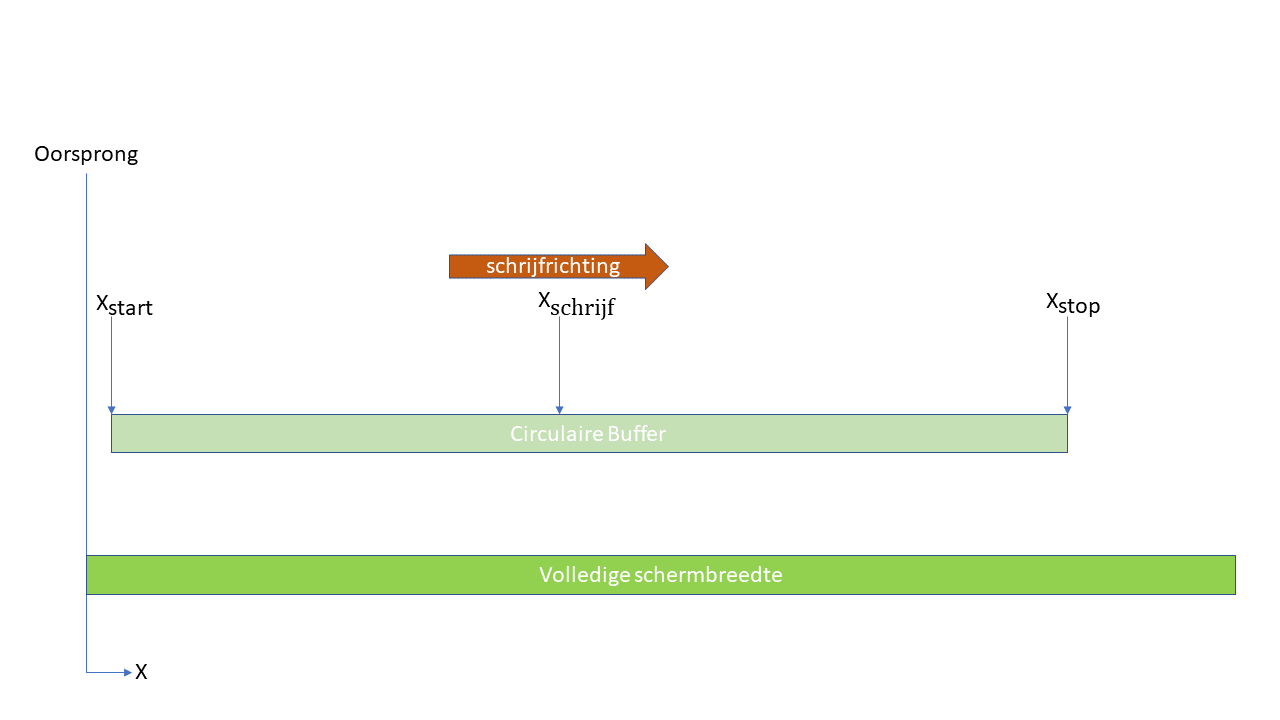
\includegraphics[width=0.7\linewidth]{leesAdressering.png}
	\caption{schematische representatie van de adressering}
	\label{fig:leesAdressering}
\end{figure}

leesAdressering

	Deze formules kunnen afgeleid worden uit de figuur \ref{fig:leesAdressering}
	\\
	
	Als $X_{VGA} < X_{stop} - X_{schrijf} + X_{start}$ dan 
	$$X_{read} = X_{VGA} + X_{schrijf} - X_{start}$$
	anders
	$$X_{read} = X_{VGA} + X_{schrijf} - X_{stop} - 2$$
	
	
	Bemerk: omdat $X_{schrijf}$ kan veranderen terwijl 1 frame van het scherm wordt opgebouwd, hebben we enkel gekeken in het begin van het scherm, en dan een vaste waarde genomen voor $X_{schrijf}$ de rest van dit frame. Om nu het effectieve adres te berekenen waar gelezen moet worden in het circulair-buffer-gedeelte, gebruiken we de volgende formule:
	$$ A_{lees} = X_{read} + lijnbreedte \times Y_{VGA} $$
	
	De data die uit dit geheugen komt is in de range 0-75 en representeert de kleur van een pixel. Om deze waarde dan effectief om te zetten naar een kleur, wordt dit getal dan via onze \textit{colorspace-vector} omgezet naar 4 bits per kleur (Rood, Groen en Blauw).

\end{itemize}

\section{Besluit}

Het is ons gelukt om een spectrogram op een extern scherm af te beelden die real-time de data verwerkt. Alle minimum vereisten zijn voldaan. We hebben gekozen om met een Zedboard te werken en om het scherm aan te sturen via VGA. Er is een interface met de audiocodec chip en de FFT wordt berekend op real-time waarden.\\

Er zijn ook enkele uitbreidingen die we hebben kunnen implementeren: het spectrogram is 3D (de amplitude van de data wordt aangegeven met kleuren) en er is een audio loopback geïmplementeerd. De audio wordt als stereo binnengelezen, maar als mono signaal doorgegeven aan de FFT controller. Dit project zou dus nog kunnen uitgebreid worden door er een stereo spectrogram van te maken. Verder zou de FFT ook kunnen berekend worden op overlappende tijdssignalen en het scherm zou kunnen uitgebreid worden naar full HD.\\

In figuur \ref{fig:spectrogram_leeg} staat het scherm van het spectrogram die wij gemaakt hebben wanneer er geen geluid aan de audiocodec gegeven wordt. \\
In figuur \ref{fig:spectrogram_chirp} staat het scherm wanneer een chirp signaal aan de audiocodec aangeboden wordt.

\begin{figure}[H]
	\centering
	\begin{subfigure}{.5\textwidth}
		\centering
		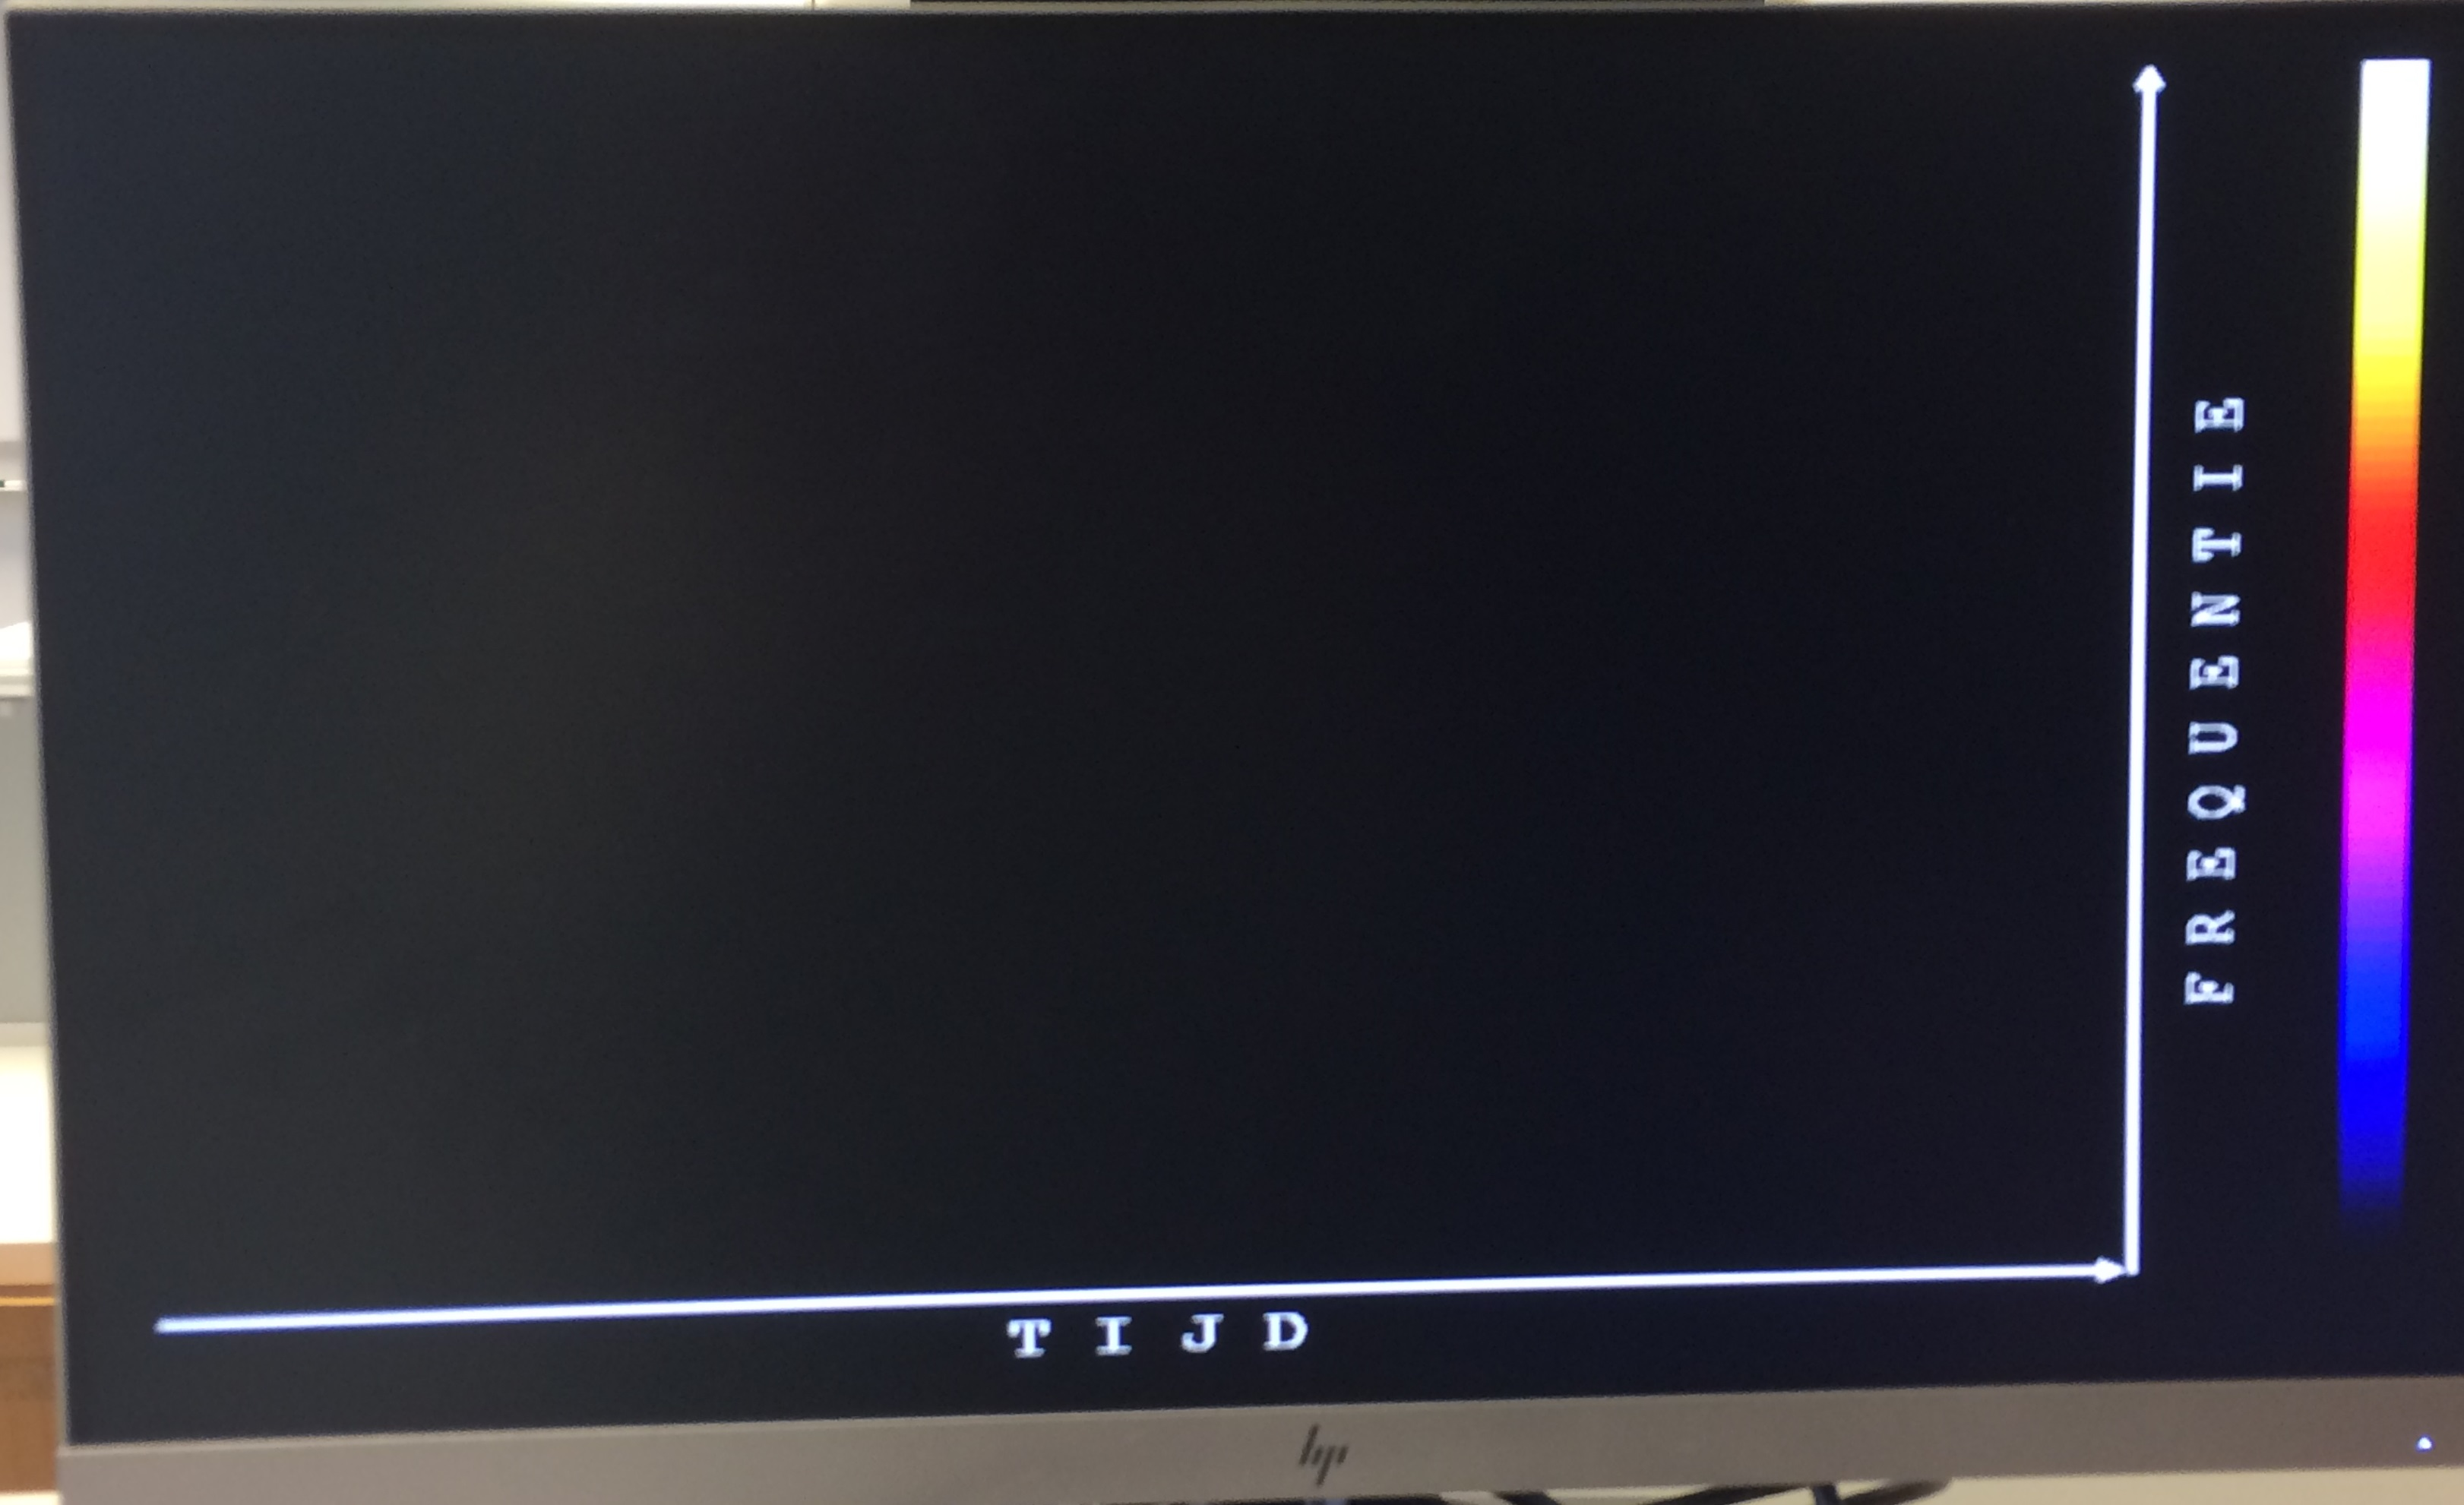
\includegraphics[width=0.9\linewidth]{Spectrogram_leeg.jpg}
		\caption{Spectrogram}
		\label{fig:spectrogram_leeg}
	\end{subfigure}%
	\begin{subfigure}{.5\textwidth}
		\centering
		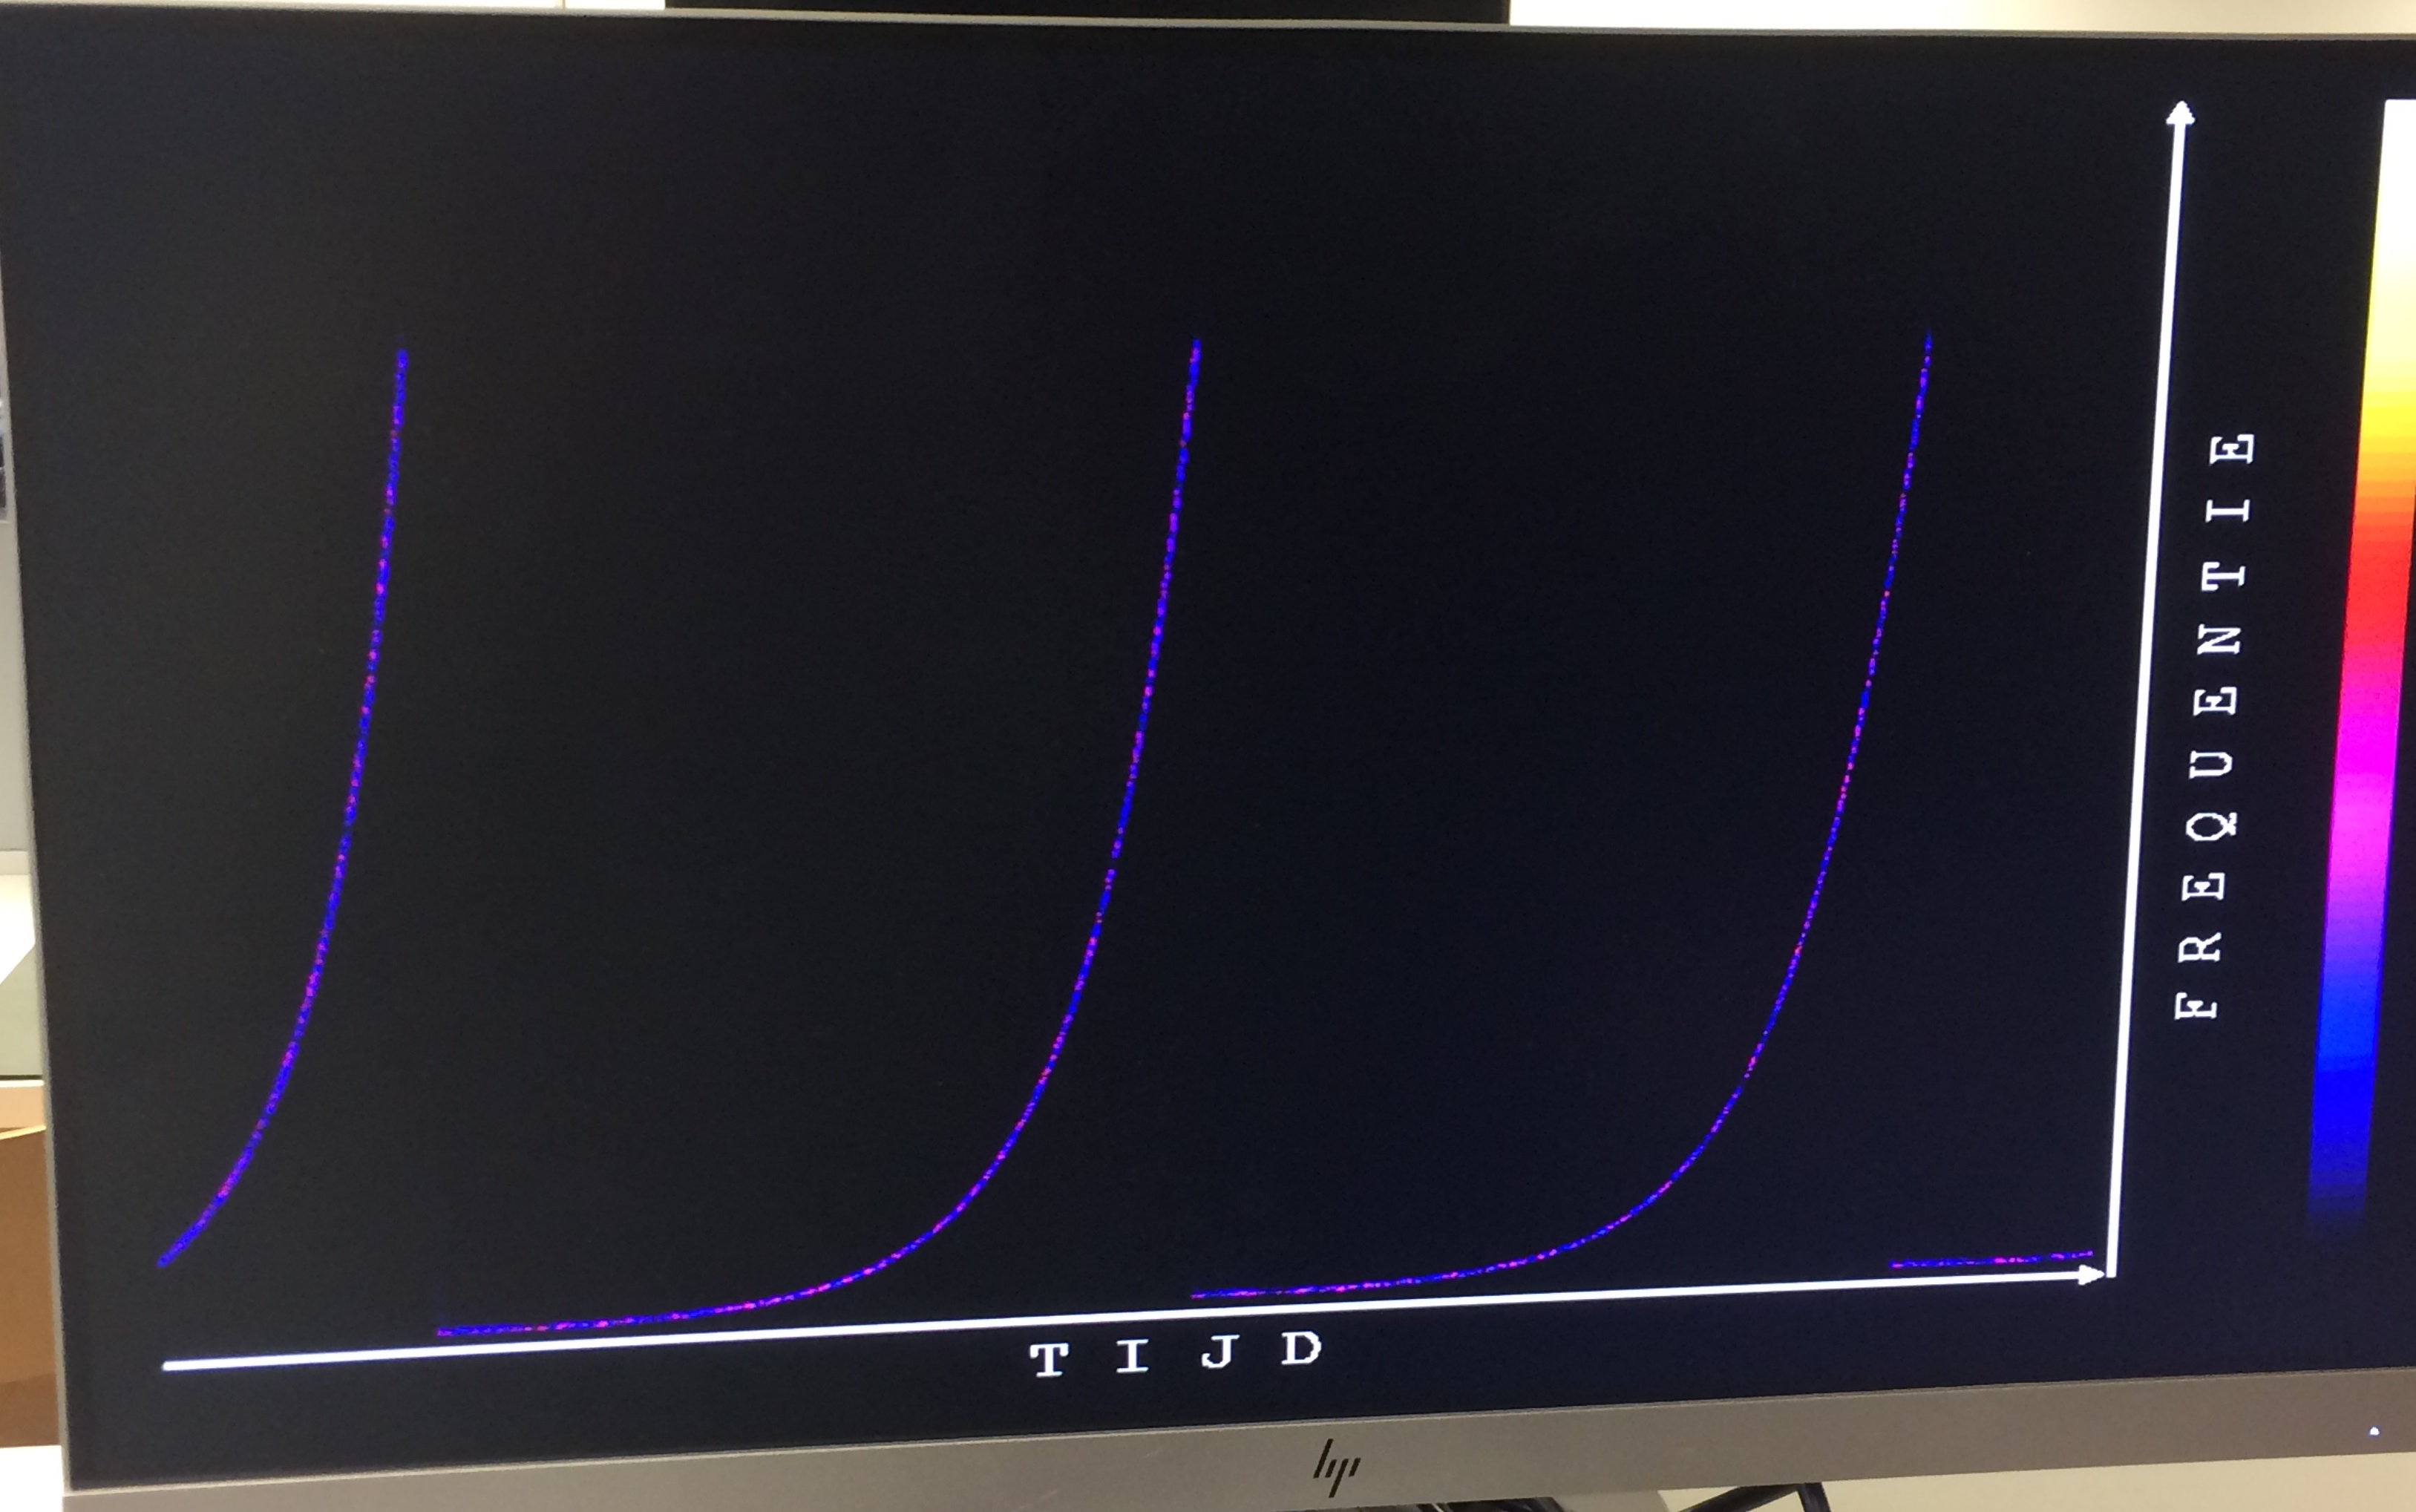
\includegraphics[width=0.9\linewidth]{Spectrogram_chirp.jpg}
		\caption{Spectrogram met chirp signaal}
		\label{fig:spectrogram_chirp}
	\end{subfigure}
	
\end{figure}

\end{document}
